\documentclass[t,compress,11pt,xcolor=dvipsnames,pdf,english]{beamer}

\usepackage[english]{babel}
\selectlanguage{english}
\usepackage[utf8]{inputenc}
\usepackage{algorithm,algorithmic}
\usepackage{graphicx,lmodern}
\usepackage{mwe}
\usepackage{caption}
\mode<presentation> {

% The Beamer class comes with a number of default slide themes
% which change the colors and layouts of slides. Below this is a list
% of all the themes, uncomment each in turn to see what they look like.

\usetheme{default}
%\usetheme{AnnArbor}
%\usetheme{Antibes}
%\usetheme{Bergen}
%\usetheme{Berkeley}
%\usetheme{Berlin}
%\usetheme{Boadilla}
%\usetheme{CambridgeUS}
%\usetheme{Copenhagen}
%\usetheme{Darmstadt}
%\usetheme{Dresden}
%\usetheme{Frankfurt}
%\usetheme{Goettingen}
%\usetheme{Hannover}
%\usetheme{Ilmenau}
%\usetheme{JuanLesPins}
%\usetheme{Luebeck}
%\usetheme{Madrid}
%\usetheme{Malmoe}
%\usetheme{Marburg}
%\usetheme{Montpellier}
%\usetheme{PaloAlto}
%\usetheme{Pittsburgh}
%\usetheme{Rochester}
%\usetheme{Singapore}
%\usetheme{Szeged}
%\usetheme{Warsaw}

% As well as themes, the Beamer class has a number of color themes
% for any slide theme. Uncomment each of these in turn to see how it
% changes the colors of your current slide theme.

%\usecolortheme{albatross}
%\usecolortheme{beaver}
%\usecolortheme{beetle}
%\usecolortheme{crane}
%\usecolortheme{dolphin}
%\usecolortheme{dove}
%\usecolortheme{fly}
%\usecolortheme{lily}
%\usecolortheme{orchid}
%\usecolortheme{rose}
%\usecolortheme{seagull}
%\usecolortheme{seahorse}
%\usecolortheme{whale}
%\usecolortheme{wolverine}

%\setbeamertemplate{footline} % To remove the footer line in all slides uncomment this line
%\setbeamertemplate{footline}[page number] % To replace the footer line in all slides with a simple slide count uncomment this line

%\setbeamertemplate{navigation symbols}{} % To remove the navigation symbols from the bottom of all slides uncomment this line
}

\usepackage{graphicx} % Allows including images
\usepackage{booktabs} % Allows the use of \toprule, \midrule and \bottomrule in tables

%----------------------------------------------------------------------------------------
%	TITLE PAGE
%----------------------------------------------------------------------------------------

\title{A GRASP-based search technique for scheduling travel-optimized warehouses in a logistics company} % The short title appears at the bottom of every slide, the full title is only on the title page

\author{Christian Pérez, Miguel A. Salido} % Your name
\institute[UPV] % Your institution as it will appear on the bottom of every slide, may be shorthand to save space
{
Universitat Politécnica de Valencia \\ % Your institution for the title page
\medskip
\textit{cripeber@upv.es, msalido@dsic.upv.es} % Your email address
}
\date{} %Date, can be changed to a custom date

\begin{document}

\begin{frame}[c]{ }
    \titlepage % Print the title page as the first slide
    \end{frame}

\begin{frame}[c]{ }
\frametitle{Overview} % Table of contents slide, comment this block out to remove it
\tableofcontents % Throughout your presentation, if you choose to use \section{} and \subsection{} commands, these will automatically be printed on this slide as an overview of your presentation
\end{frame}

%----------------------------------------------------------------------------------------
%	PRESENTATION SLIDES
%----------------------------------------------------------------------------------------

%------------------------------------------------
\section{Introduction}
%------------------------------------------------

\begin{frame}[c]{ }
    \frametitle{Introduction}
    \begin{figure}
        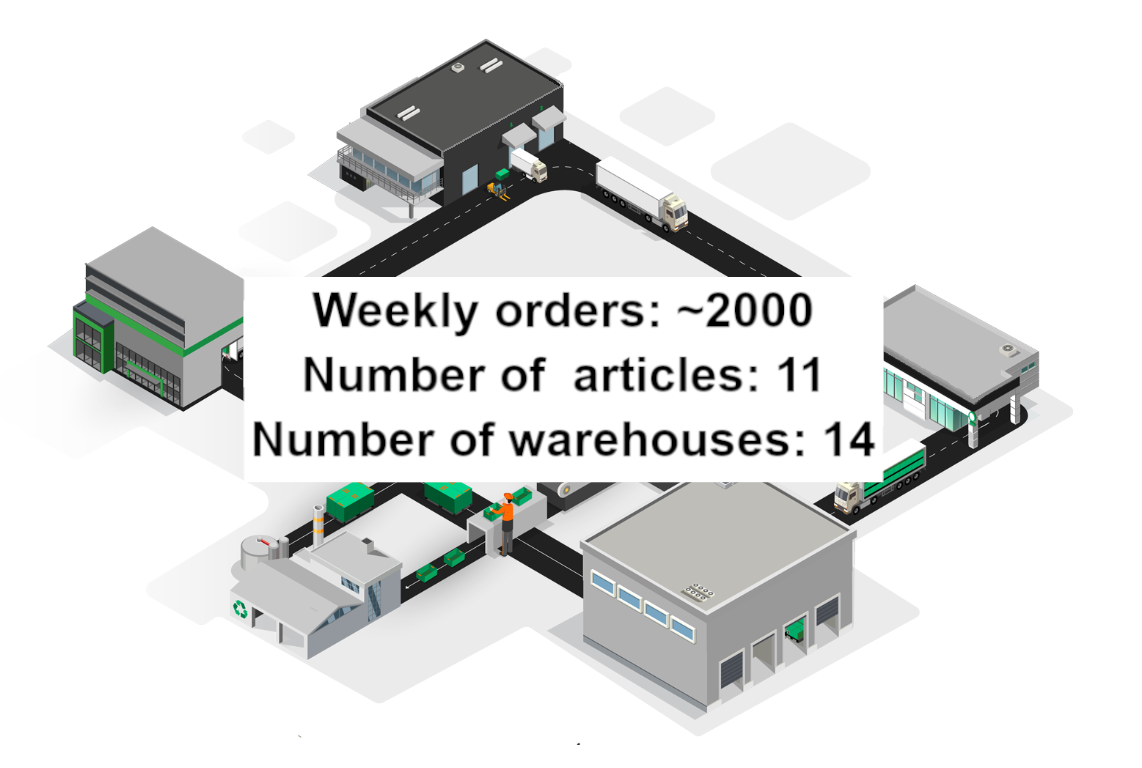
\includegraphics[width=10cm]{img/map_data.png}
        \centering
        \caption{Weekly data management by the company.}
    \end{figure}
\end{frame}

\begin{frame}[c]{ }
\frametitle{Introduction}
\begin{figure}
    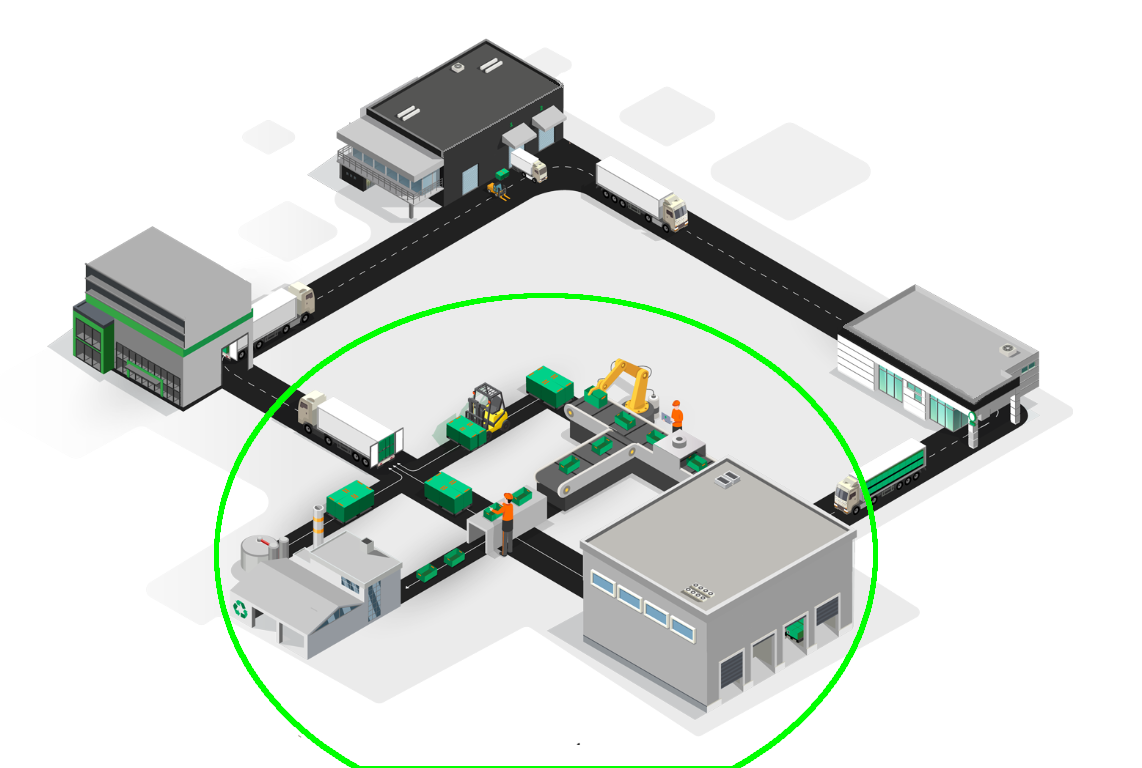
\includegraphics[width=10cm]{img/map_inner.png}
    \centering
    \caption{Diagram of the inner operation of the company.}
\end{figure}
\end{frame}

\begin{frame}[c]{ }
\frametitle{Introduction}
\begin{figure}
    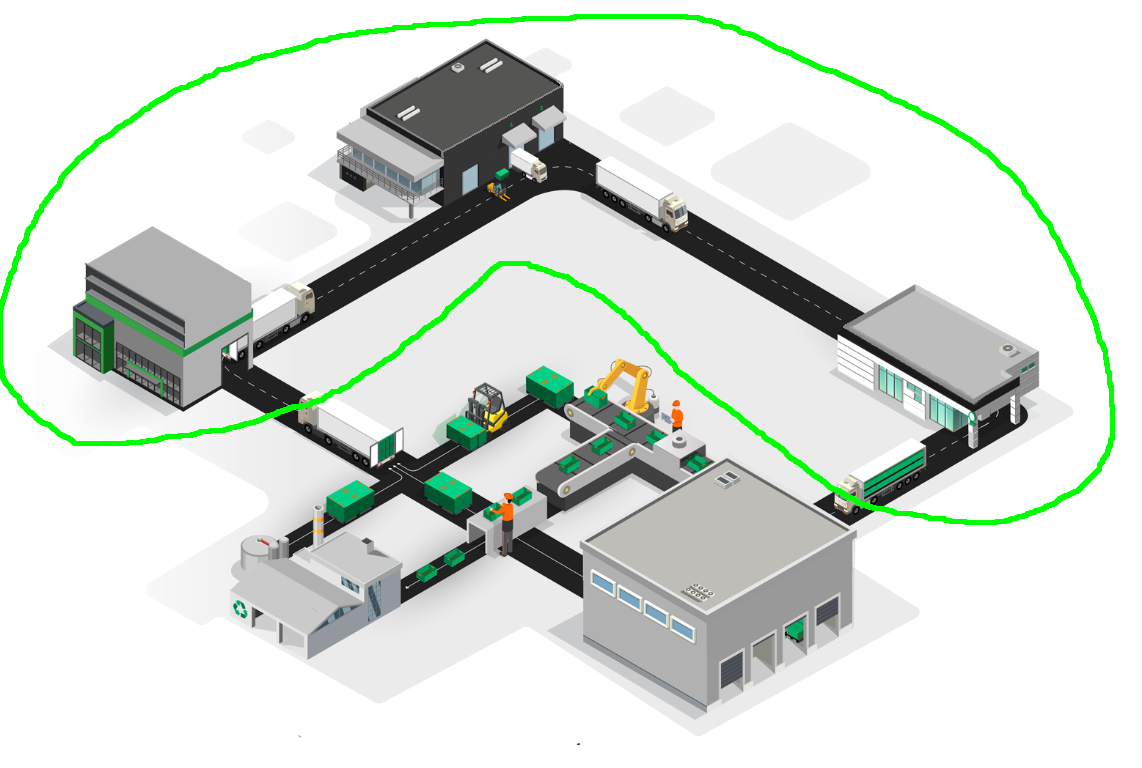
\includegraphics[width=10cm]{img/map_outter.png}
    \centering
    \caption{Diagram of the outter operation of the company.}
\end{figure}
\end{frame}


% \begin{frame}[c]{ }
% \frametitle{Introduction}
% The search techniques used by logistics companies are based on simple parameters as:
% \vspace{\baselineskip}
% \begin{itemize}
%     \item Transport cost 
%     \item Delivery time
%     \item Client specifications
% \end{itemize}
% \vspace{\baselineskip}
% However, most of them do not take into account the cost of the stock and its optimization.
% \end{frame}


%------------------------------------------------
\section{Problem specification}
%------------------------------------------------

\begin{frame}[c]{ }
    \frametitle{Problem specification}
    
    \vspace{\baselineskip}
    \begin{itemize}
        \item $DS = \{O, W, P\}$ is a triple with the weekly data of the company.
        \item $O = \{o_1, o_2, \dots, o_N \}$ is a set of orders.
        \begin{itemize}
            \item Each $o_i$ is composed by $(D_{o_i},Ir_{o_i},Ware_{o_i})$
            \item $D_{o_i}$ is the delivery date.
            \item $Ir_{o_i}$ is a set of articles to be loaded.
            \item $Ware_{o_i}$ is a set of posible warehouses.
            \begin{itemize}
                \item Each $Ware_{{o_i}j}$ is composed by $(ava_{o_{i}j},pr_{o_{i}j}, dl_{o_{i}j})$.
            \end{itemize}
        \end{itemize}

    \end{itemize}
    
\end{frame}

\begin{frame}[c]{ }
\frametitle{Problem specification}

\vspace{\baselineskip}
\begin{itemize}
    \item $W = \{w_1, w_2, w_3, \dots w_M \}$ is a set of warehouses
    \begin{itemize}
        \item Each warehouse $w_i$ is a bidirection matrix.
        \item The rows refers to an article.
        \item The column refers to a day of week.
        \item $w_{ijk} \in \mathbb{N}$
    \end{itemize}
    \item $P = \{p_1, p_2, p_3, \dots p_P \}$ is a set of prices

\end{itemize}

\end{frame}

\begin{frame}[c]{ }
    \frametitle{Objective function}

        \begin{itemize}
            \item $f \longleftarrow \alpha * Ct + (1 - \alpha) * \sum Cs$
            \item $Ct :$ Variable that contains the transport cost of a warehouse order tuple.
            \item $Cs :$ List containing the stock cost of each of the items in the order for a specific warehouse.
            \item $\alpha :$ [0 - 1]

        \end{itemize}

\end{frame}
%------------------------------------------------
\section{Solving techniques}

%------------------------------------------------

\begin{frame}[c]{ }
\frametitle{Solving techniques}
    \large
    The Greedy algorithm provided by the company
    \normalsize
    
    \begin{itemize}
        \item Control of the distance from the warehouse to the customer and other convenient factors.
        \item The zone of influence or geographical area is a higher priority in the assignment.
        \item Restrict the warehouses loading by the type of articles contained in the order.
        \item The quantity of articles is not constant throughout the year.
    \end{itemize}
\end{frame}


\begin{frame}[c]{ }
\frametitle{Solving techniques}
    \large
    GRASP
    \small

    \begin{algorithmic}[1]
        \STATE \textbf{\emph{input:}} Orders $O$, Stocks matrix $W$, Article price vector $P$, Size of LCR list $n$
        \STATE \textbf{\emph{output:}} Optimized solution $s^*$
        
        \STATE $s \longleftarrow [\quad] $
        \STATE $LCR \longleftarrow \textbf{LCRordening}(O, n)$
        \STATE \textbf{while } $|s| \neq |LCR|$ \textbf{do}:\label{1grasp}
        \STATE \quad $j \longleftarrow 0 $
        \STATE \quad $lcr \longleftarrow [\quad]$
        \STATE \quad \textbf{while } $j < |LCR|$ \textbf{do}:
        \STATE \quad \quad $lcr \longleftarrow lcr \cup \textbf{LocalSearch}(LCR_j,\alpha,|LCR|)$
        \STATE \quad \quad $j \longleftarrow j + 1$
        \STATE \quad $\textbf{end while}$
        \STATE \quad $s \longleftarrow s \cup lcr*$ 
        \STATE \quad $LCR \longleftarrow (LCR \setminus lcr*) \cup  LCR_{n+1} $ 
        \STATE $\textbf{end while}$\label{2grasp}
        \STATE \textbf{return }$s$
    \end{algorithmic}
\end{frame}

\begin{frame}[c]{ }
    \frametitle{Solving techniques}
    \large
    Local Search
    \small

    \begin{algorithmic}[1]
        \STATE \textbf{\emph{input:}} A order $o$, List of item price $P$, Alpha value for objective function $\alpha$, Length of LCR list $nLCR$
        \STATE \textbf{\emph{output:}} Index of warehouse chosen $j$, Minimum cost of warehouse chosen $Q*$
        \STATE  $Q \longleftarrow [\quad]$
        \STATE  $I \longleftarrow Ir_{o}, M \longleftarrow W_{o}$
        \STATE  \textbf{For} $j$ \textbf{in} $\{ 0,\dots,|M|\}$:
        \STATE  \quad $Cs \longleftarrow [\quad]$
        \STATE  \quad $Ct \longleftarrow \textbf{getTransportCost}(M_j) $
        \STATE  \quad \textbf{For} $i$ \textbf{in} $\{ 0,\dots,|I|\}$:
        \STATE  \quad \quad$Cs \longleftarrow Cs \cup P_i * \sum_{k=D_{o}}^{|wst_{ij}|} wst_{ijk}\; |\; wst_{ijk} < 0 $
        \STATE  \quad  $\textbf{end for}$
        \STATE  \quad $Q_j \longleftarrow \alpha * Ct + (1 - \alpha) * \sum Cs$
        \STATE  \quad $Q \longleftarrow Q \cup Q_j$
        \STATE  \quad $\alpha \longleftarrow \textbf{AlphaScheduler}(Cs) $
        \STATE  $\textbf{end for}$
        \STATE  \textbf{return }$\left( min(Q) , Q_{min(Q)} \right)$
    \end{algorithmic}
\end{frame}

    
%------------------------------------------------
\subsection{Ordering heuristics}
%------------------------------------------------

\begin{frame}[c]{ }
    \frametitle{Ordering heuristics}
    \begin{figure}
        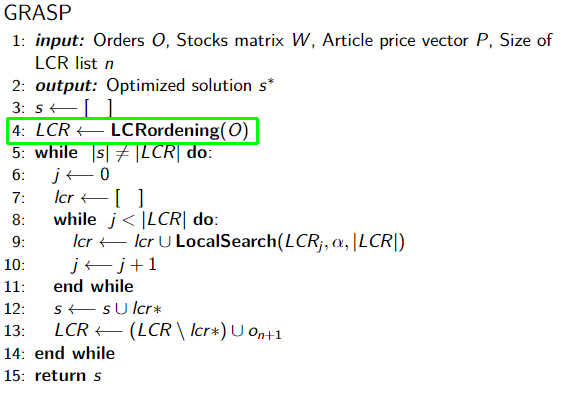
\includegraphics[width=11cm]{img/GRASPALGO_ordening.png}
        \centering
    \end{figure}        
\end{frame}

\begin{frame}[c]{ }
    \frametitle{Ordering heuristics}
    \begin{block}{LCR ordering}
        {
            The ordering of the LCR list depending on a number of characteristics of the orders:
            \begin{itemize}
                \item Number of available warehouses (Model 1)
                \item Number of warehouses and articles (Model 2)
                \item Number of warehouses and delay (Model 3)
                \item Number of warehouses and standarized dealy and articles (Model 4)
                \item Number of weight warehouses and delay (Model 5)
                \item Early dealy and number of articles (Model 6)
            \end{itemize}
        }
    \end{block}
\end{frame}


%------------------------------------------------
\subsection{Improvements}
%------------------------------------------------

    \begin{frame}[c]{ }
    \frametitle{Improvements}
    \begin{block}{Shuffle}
        {
            This method randomize the LCR list from the criteria used in LCR ordening.
            \begin{figure}
                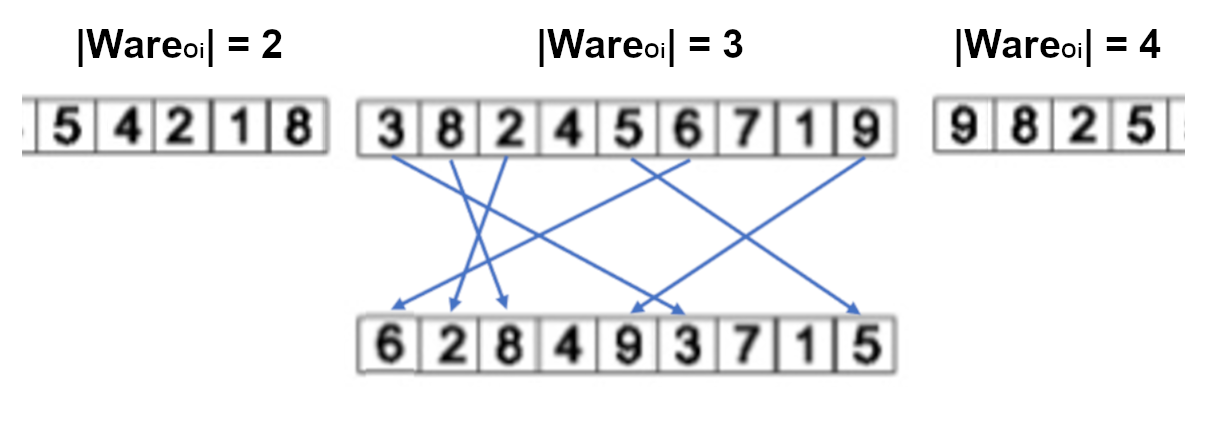
\includegraphics[width=10cm]{img/shuffle.png}
                \centering
                \caption{Example of randomize shuffle method}
            \end{figure}
            
        }
    \end{block}

\end{frame}

\begin{frame}[c]{ }
    \frametitle{Improvements}
    \begin{figure}
        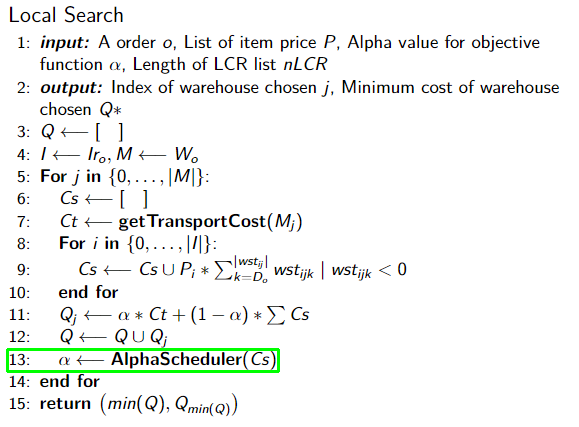
\includegraphics[width=11cm]{img/LOCALALGO_1.png}
        \centering
    \end{figure}        
\end{frame}

\begin{frame}[c]{ }
    \frametitle{Improvements}
    \begin{block}{Alpha scheduler}
        {
            It is observed that alpha value polarize fitness function during the execution tests.

            Increases or decreases the alpha variable regardless of whether or not the assigned order is in a warehouse with negative stock.
        }
    \end{block}

    \vspace{\baselineskip}

    \begin{figure}[ht]
        \centering
        \begin{minipage}{0.5\linewidth}
            \begin{algorithmic}[H]
                \STATE  $F_{\alpha}  \longleftarrow (1-\alpha) / nLCR$ 
                \STATE
                \STATE  \textbf{if} $\sum Cs \leqslant 0$ \textbf{then}:
                \STATE  \quad $\alpha \longleftarrow \alpha + F_{\alpha}$
                \STATE  $\textbf{else:}$
                \STATE  \quad $\alpha \longleftarrow \alpha - F_{\alpha}$
                \STATE  $\textbf{end if}$
            \end{algorithmic}
        \end{minipage}
    \end{figure}

\end{frame}


%------------------------------------------------
\section{Evaluation}
%------------------------------------------------

\begin{frame}[c]{ }
    \frametitle{Evaluation}
    \begin{block}{Study cases}
        {
            We manage three cases provided by the company:
            \begin{itemize}
                \item \textbf{Test case:} dataset prepared by the company to test the algorithm. This data set is used to tune the parameters of the GRASP algorithm.
                \item \textbf{Study cases:} dataset with orders for the first and second week of July  
            \end{itemize}
        }
    \end{block}
    \begin{block}{Complexity}
        {
            \begin{itemize}
                \item \textbf{Orders:} $\simeq$ 2000
                \item \textbf{Possible warehouses in $o_i$:} [1 - 14]
                \item \textbf{Articles in $o_i$:} [1 - 11]
            \end{itemize}
        }
    \end{block}
    \end{frame}

\begin{frame}[c]{ }
    \frametitle{Evaluation}
        \begin{figure}[H]
            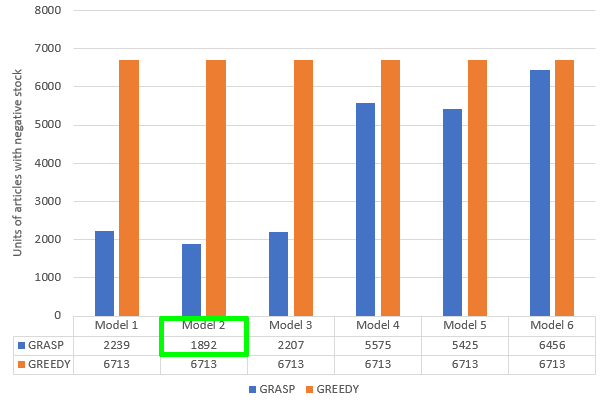
\includegraphics[ width=10cm]{img/dispersionMODEL.png}
            \centering
            \caption{Dispersion of negative stock for each model.}
        \end{figure}
    \end{frame}

\begin{frame}[c]{ }
    \frametitle{Evaluation}
        \begin{figure}[H]
            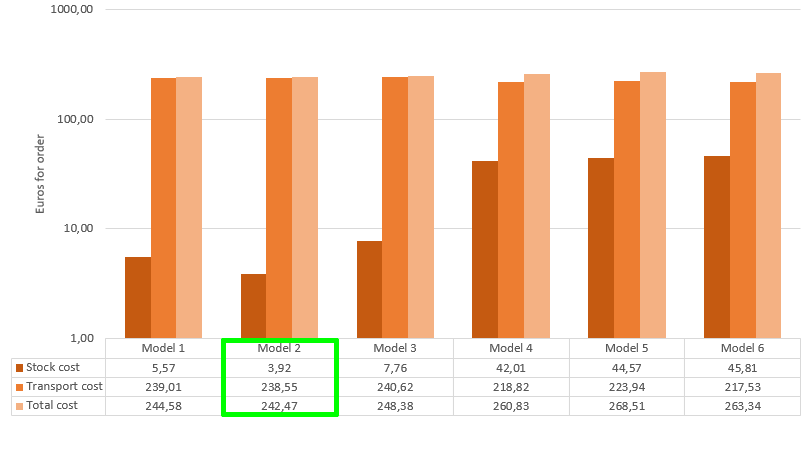
\includegraphics[width=10cm]{img/costcomparisionMODEL.png}
            \centering
            \caption{Cost comparison for each model.}
        \end{figure}
    \end{frame}

% \begin{frame}[c]{ }
%     \frametitle{Evaluation}
%         \begin{figure}[H]
%             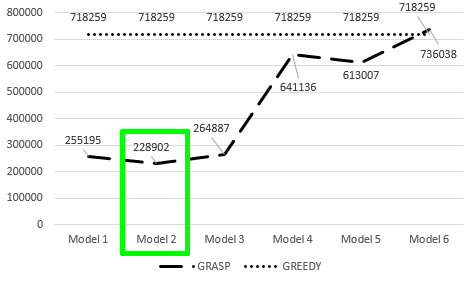
\includegraphics[ width=10cm]{img/averagestocknegativeMODEL.png}
%             \centering
%             \caption{Average of articles with negative stock for each model}
%         \end{figure}
%     \end{frame}

% \begin{frame}[c]{ }
% \frametitle{Evaluation}
%     \begin{figure}[H]
%         \centering
%         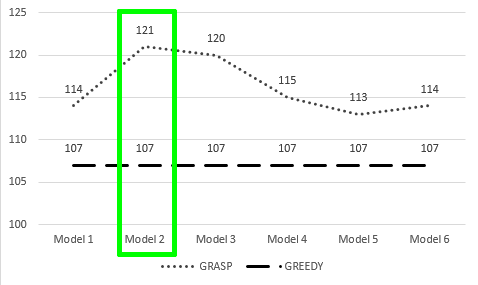
\includegraphics[ width=\linewidth]{img/itemsstocknegativeMODEL.png}
%         \caption{Quantity of articles with negative stock for each
%         model}
%     \end{figure}
% \end{frame}


% \begin{frame}[c]{ }
% \frametitle{Evaluation}

% \begin{figure}[H]
%     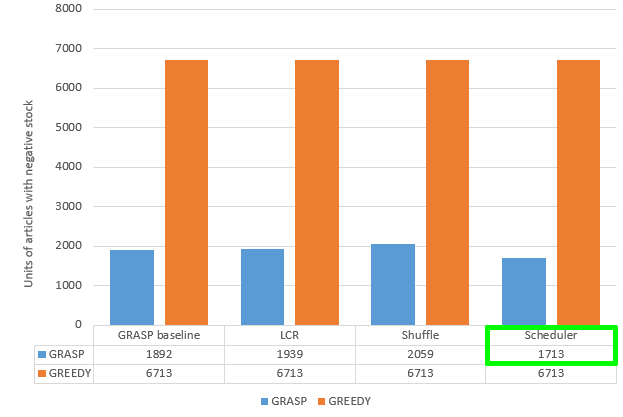
\includegraphics[ width=10cm]{img/dispersionIMPROV.png}
%     \centering
%     \caption{Dispersion of negative stock for each improvement.}
% \end{figure}

% \end{frame}

\begin{frame}[c]{ }
    \frametitle{Evaluation}
    \begin{figure}[H]
        \centering
        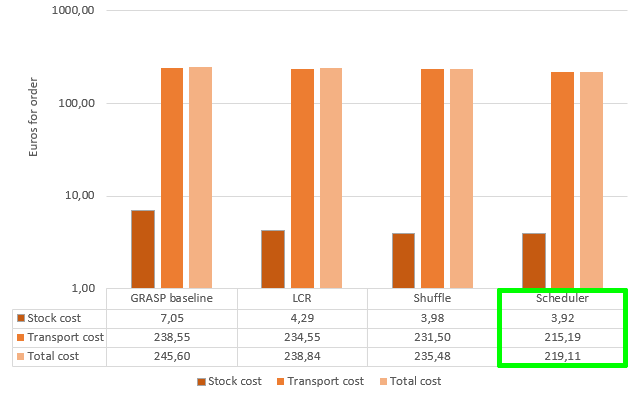
\includegraphics[width=10cm]{img/comparisoncostIMPROV.png}
        \caption{Different costs for each improvement.}
    \end{figure}
\end{frame}

\begin{frame}[c]{ }
    \frametitle{Evaluation}
    \begin{figure}[H]
        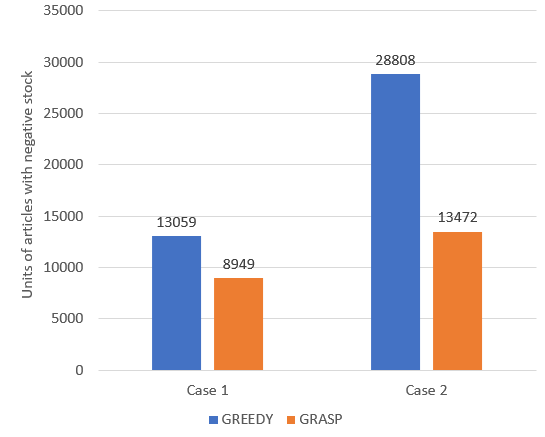
\includegraphics[ width=9cm]{img/dispersionALGOTH.png}
        \centering
        \caption{Dispersion of negative stock for case study.}
    \end{figure}
    
\end{frame}
    
\begin{frame}[c]{ }
    \frametitle{Evaluation}
    \begin{figure}[H]
        \centering
        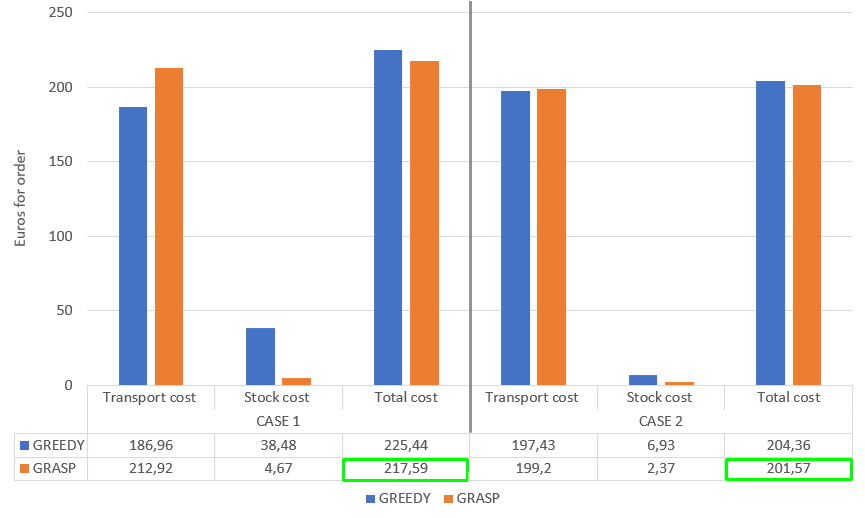
\includegraphics[width=10cm]{img/costcomparisionALGOTH.png}
        \caption{Different costs for each case study.}
    \end{figure}
\end{frame}

%------------------------------------------------
\section{Conclusions and future work}
%------------------------------------------------

\begin{frame}[c]{ }
    \frametitle{Conclusions and future work}
    \begin{block}{Conclusions}
        {
            \begin{itemize}
                \item Logistic companies need to optimize their strategies to be more efficient.
                \item This paper shows that two problems can be combined: the warehouse stock management and routing problem.
                \item GRASP-based metaheuristic improve the negative average stock by up to 82\%.
                \item Current tools cannot find a solution in a reasonable time. 
                \item The proposed developed algorithm obtains a optimized solution in less than 1.5 minutes.
            \end{itemize}
        }
    \end{block}
    \begin{block}{Future work}
        {
            \begin{itemize}
                \item Create a data pool from the grasp-based metaheuristic solutions.
                \item Develop a genetic algorithm where the initial population is fed with solutions obtained by GRASP.
            \end{itemize}
        }
    \end{block}
\end{frame}

\begin{frame}[c]{ }
    \titlepage % Print the title page as the first slide
\end{frame}

\end{document}